% !TEX root = ../notes_missingsemester.tex
% Chapter 9: Watch It Run — Monitoring, Logging & Analytics
%%%%%%%%%%%%%%%%%%%%%%%%%%%%%%%%%%%%%%%%%%%%%%%%%%%%%%%%%%%%%%%%%%%%%%

% POST IMPROVEMENTS 2026:
% 1. Add a TikZ figure of the alert path from probe to Discord channel.
% 2. Provide a pre-baked v0.7 reference repo so catch-up takes a single clone.

\index{monitoring}\index{logging}\index{analytics}\index{Discord webhook}\index{journalctl}\index{observability}\index{structured logging}\index{request ID}\index{health probe}\index{alerting}\index{jq}
\chapter{Watch It Run: Monitoring, Logging \& Analytics}
\printchapterversion{09_monitoring_logging}
\newthought{You cannot improve what you cannot measure.}

% ==============================================================================================
% BLOCK 1: INTRODUCTION
% ==============================================================================================

\section{The Why}\index{observability}\index{operations}

Block~8 left us with a service that ships itself. Continuous integration
runs lint and tests on every push, continuous deployment to \texttt{prod}
happens on every merge to \texttt{main}, a cron job snapshots the
database every night, and a \texttt{MODEL\_VERSION} flag toggles which
classifier the handler loads. The pipeline runs. The service deploys.
Backups land in a tarball. What none of it does is tell us whether the
running service is healthy, what it is doing, who is calling it, or how
the model is performing in the wild.

\newthought{Every error today is a future user complaint.}\index{PixelWise}
Every slow request is invisible until somebody happens to retry. Every
crash that systemd quietly restarts leaves no trace except a hole in the
log where the request should have been. The service is reachable on
\texttt{https://192.168.56.11}, it answers \texttt{GET /health}, and
nobody is watching. That is the gap this block closes.

\newthought{Observability is the practice} of building enough signal into
a running system that you can answer questions about its behaviour
without redeploying it. Three pillars carry the standard
definition\index{three pillars}: Logs record what happened, metrics
count how often it happened, traces show how a single request travelled
through the system. PixelWise focuses on logs and a minimum of metrics
in this block. Distributed tracing is out of scope for the lab; the
optional section at the end sketches where you would add it later.

\begin{figure}
\centering
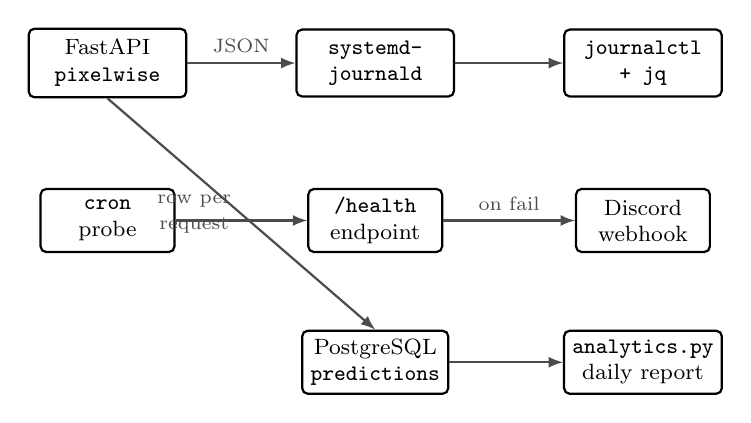
\begin{tikzpicture}[
    every node/.style={font=\footnotesize, align=center},
    box/.style={rectangle, draw=black, thick, rounded corners=2pt, minimum width=2.0cm, minimum height=0.85cm, inner sep=4pt},
    smallbox/.style={rectangle, draw=black, thick, rounded corners=2pt, minimum width=1.7cm, minimum height=0.8cm, inner sep=3pt},
    arr/.style={-latex, thick, black!70}
]
\node[box] (svc) at (0, 0)     {FastAPI\\\texttt{pixelwise}};
\node[box] (jd)  at (3.4, 0)   {\texttt{systemd-}\\\texttt{journald}};
\node[box] (jc)  at (6.8, 0)   {\texttt{journalctl}\\\texttt{+ jq}};
\node[smallbox] (cron) at (0, -2.0)  {\texttt{cron}\\probe};
\node[smallbox] (hp)   at (3.4, -2.0){\texttt{/health}\\endpoint};
\node[smallbox] (disc) at (6.8, -2.0){Discord\\webhook};
\node[smallbox] (pg)   at (3.4, -3.8){PostgreSQL\\\texttt{predictions}};
\node[smallbox] (an)   at (6.8, -3.8){\texttt{analytics.py}\\daily report};

\draw[arr] (svc.east) -- node[above]{\scriptsize JSON} (jd.west);
\draw[arr] (jd.east)  -- (jc.west);
\draw[arr] (cron.east) -- (hp.west);
\draw[arr] (hp.east)   -- node[above]{\scriptsize on fail} (disc.west);
\draw[arr] (svc.south) -- node[left]{\scriptsize row per\\\scriptsize request} (pg.north);
\draw[arr] (pg.east)   -- (an.west);
\end{tikzpicture}
\caption{The observability flow added in Block~9. The FastAPI service emits structured JSON over standard output; \texttt{systemd-journald} stores every line and \texttt{journalctl} queries it, optionally piped into \texttt{jq}. A cron-driven probe hits the \texttt{/health} endpoint every five minutes and posts to a Discord webhook on failure. The same \texttt{predictions} table from Block~6 doubles as the analytics warehouse; a small \texttt{analytics.py} script summarises it on demand.}
\label{fig:observability_flow}
\end{figure}

\newthought{Why operate, not just deploy?}
A pipeline that ships code is half the job. The other half is the running
service: Knowing that it is up, knowing what it is doing, knowing when
something has changed for the worse. A team that can deploy but cannot
observe ships faster than it can debug, which is the textbook recipe for
an outage that nobody can explain.

\newthought{Beyond this course,} the same three pillars carry production
practice. Engineers run dashboards that watch error rates, latency
percentiles, and saturation. Alerts wake on-call rotations when a
service stops behaving. Data teams query the same operational tables to
detect drift and trigger retraining. We build a small version of each
piece, enough to feel the shape of the discipline.

\newpage
\subsection{Hands On Experience}

\newthought{Consider this scenario:} A user emails on a Tuesday morning
saying the site was broken yesterday at 9pm. You have no idea. You did
not look at the service yesterday, no alert ever fired, the log lines
you would search for were never queried, and you cannot reproduce the
problem because you do not even know what request the user sent. The
service might have been down for ten minutes. The service might be down
right now. There is no way to tell from where you are sitting.

\newthought{The operational gap is the headline.}\index{operations}
A service that ships without observability is a service that fails
silently. The fix is not a new framework. It is structured logs you can
query, a request ID that ties every line of a single request together,
a probe that asks the service whether it is alive on a schedule you set,
a notification channel that wakes you when the answer is no, and a
handful of SQL queries that turn the \texttt{predictions} table into a
view of how the model is being used.

\marginnote{\newthought{Outside the classroom.}\index{operations}
Production teams build the same shape with larger tools: A central log
store like Loki or OpenSearch, a metrics database like Prometheus, a
notification fan-out through PagerDuty or Opsgenie, a tracing backend
like Jaeger, dashboards in Grafana. The pieces grow; the responsibilities
do not. Every team that runs a service answers the same questions you
will answer in this block.}

\newthought{Structured beats printed.}\index{structured logging}
A printed line is a string that a human reads. A structured line is a
JavaScript Object Notation (JSON) object that a machine can filter by
field. The difference between them is the difference between scrolling
and querying. By the end of this block the service will emit JSON, the
journal will store it, and \texttt{journalctl} piped into \texttt{jq}
will let you ask the questions that the previous blocks could not.

\newthought{This ninth block} introduces observability for PixelWise.
By the end you will have
\begin{itemize}
    \item configured structured JSON logging for the FastAPI application,
    \item written useful queries against \texttt{journalctl} to find errors and slow requests,
    \item added a request ID middleware so every log line for a single request shares an ID,
    \item built a cron-driven probe that hits the service every five minutes and pings Discord on failure,
    \item run analytics queries against the \texttt{predictions} table to see volume, distribution, and confidence over time,
    \item and tagged the result as \texttt{v0.8}.
\end{itemize}



% ==============================================================================================
\newpage
\section{Optional Exercise: Catch Up to \texttt{v0.7}}\index{exercises}\index{Git!tag}\index{recovery}

\marginnote{\newthought{Tag map.}\index{Git!tag}
\texttt{v0.7} marks the end of Block~8, \texttt{v0.8} will mark the end
of this block.
Browse the full set at
\url{https://github.com/schutera/pixelwise/tags}.}

\newthought{Catching up via tag.}\index{Git!tag}\index{recovery}
This catch-up extends the one in Block~8. If you have not done that one,
do it first: It lands you at \texttt{v0.6}, the end-of-Block~7 state.
The exercise here picks up from there and rewinds to \texttt{v0.7}, the
end-of-Block~8 state, with continuous integration running lint and tests
on every push, continuous deployment to \texttt{prod} on every merge to
\texttt{main}, a deploy script invoked by the workflow, a cron entry on
\texttt{prod} for nightly database backups, and a \texttt{MODEL\_VERSION}
feature flag read from the environment in \texttt{app/main.py}.

\newthought{Both VMs this time.} Block~8 wired automation that touches
both machines, so this catch-up brings them both to \texttt{v0.7}. The
Git-tracked changes since \texttt{v0.6} include
\texttt{.github/workflows/ci.yml} and
\texttt{.github/workflows/deploy.yml},
\texttt{deploy/deploy.sh}, \texttt{crontab.txt} for the nightly backup
schedule, the \texttt{MODEL\_VERSION} read from the environment in
\texttt{app/main.py}, and a refreshed \texttt{.env.example} with the new
flag. The local \texttt{.env} on each VM needs the new value written by
hand; \texttt{setup-server.sh} then installs the cron entry from
\texttt{crontab.txt} and restarts the service. GitHub-side state, the
repository secrets and the workflow run history, lives on GitHub itself
and is not part of the VM, so verify your secrets are still configured
rather than recreating them.

\marginnote{\newthought{Sequence on \texttt{dev}.}\\[0.4em]
\texttt{cd \textasciitilde/pixelwise}\\
\texttt{git fetch origin -{}-tags}\\
\texttt{git reset -{}-hard v0.7}\\
\texttt{cp .env.example .env}\\
\texttt{nano .env}\\
\texttt{source .venv/bin/activate}\\
\texttt{pip install -r requirements.txt}\\
\texttt{bash setup-server.sh}\\[0.3em]
Edit \texttt{.env} to set \texttt{MODEL\_VERSION} and any local
overrides. If \texttt{.venv/} is missing, run
\texttt{python3 -m venv .venv} before the \texttt{source} step.}

\newthought{Run the catch-up on \texttt{dev}.}
Rewind the repository to \texttt{v0.7}, refresh \texttt{.env} from the
updated example and edit it for any new secrets such as
\texttt{MODEL\_VERSION}, reinstall pinned dependencies if your virtual
environment was wiped, then run \texttt{setup-server.sh} to apply the
local side effects. The exact commands are in the margin.

\marginnote{\newthought{Sequence on \texttt{prod}.}\\[0.4em]
\texttt{ssh produser@192.168.56.11}\\
\texttt{cd /opt/pixelwise}\\
\texttt{git fetch origin -{}-tags}\\
\texttt{git reset -{}-hard v0.7}\\
\texttt{cp .env.example .env}\\
\texttt{nano .env}\\
\texttt{source .venv/bin/activate}\\
\texttt{pip install -r requirements.txt}\\
\texttt{bash setup-server.sh}\\[0.3em]
Then from \texttt{dev}:
\texttt{curl http://192.168.56.11:8000/health}
should return \texttt{\{"status":"ok"\dots\}}.}

\newthought{Run the catch-up on \texttt{prod}.}
Same sequence on \texttt{prod}, where \texttt{setup-server.sh} also
installs the cron entry from \texttt{crontab.txt} and restarts the
service. After the script finishes, verify the API is reachable from
\texttt{dev}.

\marginnote{\newthought{Already have a fork?}\index{Git!fork}
If your own fork carries the \texttt{v0.7} tag, swap \texttt{origin} on
\texttt{dev} with
\texttt{git remote set-url origin git@github.com:<you>/pixelwise.git}
so push and pull continue to target your account. The HTTPS clone on
\texttt{prod} stays read-only. Verify your GitHub repository secrets
are still configured on the fork; they live with the repository on
GitHub, not in the VM.}

\newthought{You are now} at the state where Block~8 ended, with both
machines aligned, ready to start Block~9.



% ==============================================================================================
% BLOCK 2: CONCEPTS AND PRACTICE
% ==============================================================================================

\newpage
\section{The Three Pillars of Observability}\index{observability}\index{logs}\index{metrics}\index{traces}

\newthought{Logs are events.}\index{logs}
Each line records that something happened: A request arrived, a query
ran, a handler raised. A log line has a timestamp, a level, and a
message body. Structured logs add named fields so you can filter by
endpoint, by status, by request identifier (ID), or by anything else
the application attaches at write time. Logs answer: What happened, and
when?

\newthought{Metrics are counts.}\index{metrics}
A metric is a number with a name and a set of labels, updated over time.
Request count per endpoint, error count per status code, latency
percentile per route. Metrics answer: How often, how fast, how many?
They are cheap to store because they aggregate; a million requests
become a single counter.

\marginnote{\newthought{Why focus on logs first?}\index{logs}
A small service in a single VM can get most of its operational visibility
from logs alone. You can grep for errors, filter for slow requests, and
correlate by request ID. Metrics shine when you have many services and
need a dashboard; they are not free, so it makes sense to add them after
logs, not before.}

\newthought{Traces are paths.}\index{traces}
A trace follows one request as it crosses service boundaries: The HTTP
hop into the API, the SQL query to the database, the call out to the
model artefact, the response back. Each step is a span; spans nest;
the trace is the tree. Traces answer: Where did the time go for this
specific request? They become essential once a request touches more
than one service, and overkill before that point. The PixelWise service
is one process behind one reverse proxy, so we leave tracing for later.

\newthought{The pillar names a question, not a tool.}\index{observability}
The same JSON line can be a log to one consumer, a metric to another,
and a span to a third. What changes is what you do with the line, not
the line itself. The exercises below put the JSON on the wire and let
\texttt{journalctl} be the first consumer.

\marginnote{\newthought{Out of scope for this lab.}\index{tracing}
Distributed tracing with OpenTelemetry is the production standard for
the third pillar, and a worthwhile detour for any student curious about
it. The shape is familiar from this block: A library in the service
emits trace data, a collector receives it, a backend stores it, a
viewer renders it. The optional section at the end sketches where it
slots in.}



% ==============================================================================================
\newpage
\section{Structured Logging in Python}\index{structured logging}\index{logging}

\newthought{Printing strings is technical debt.}\index{logging}
A line like \texttt{print("got request")} tells you that something
happened. It does not tell you what endpoint was hit, what request ID
the call carried, how long the handler took, or what the response code
was. You cannot filter by status code if the status code is not a
field. You cannot find every slow request if the latency is buried in
prose. Every later question becomes a regular expression on free-form
text, which is the operational equivalent of grepping a textbook.

\newthought{Structured logging} writes each event as a JSON object on a
single line. The object has a fixed set of top-level keys: timestamp,
level, logger name, message, and any extra fields the call site
attaches. The line is one piece of valid JSON; \texttt{jq} can filter
it, a log shipper can route it, an aggregation tool can index it.
Humans can still read it, especially if the formatter pretty-prints on
a terminal and compacts on a pipe.

\marginnote{\newthought{What the JSON line looks like.}\index{JSON}
A representative line from the service after this block:
{\footnotesize\begin{verbatim}
{"ts":"2026-04-05T14:23:01Z",
 "level":"INFO",
 "logger":"pixelwise.api",
 "msg":"classify ok",
 "request_id":"abc-123",
 "endpoint":"/classify",
 "status":200,
 "latency_ms":42,
 "model_version":"v1",
 "predicted_class":"7",
 "confidence":0.94}
\end{verbatim}}
Every field is queryable. Compare with the equivalent printed string,
which is queryable only with a regex you would have to maintain.}

\newthought{Python's \texttt{logging} module} is the standard library
plumbing for this. A \texttt{Logger} produces \texttt{LogRecord}
objects, a \texttt{Formatter} turns each record into a string, a
\texttt{Handler} writes the string somewhere. To emit JSON, you write
a custom \texttt{Formatter} that serialises the record as JSON instead
of formatting it as text. Everything else stays the same: The
application code still calls \texttt{logger.info("classify ok",
extra=\{...\})} and the formatter handles the rest.

\newthought{Uvicorn has its own loggers.}\index{uvicorn}
The HyperText Transfer Protocol (HTTP) server emits an access log line
per request and an error log line per failure, both as plain text by
default. To make the whole service speak JSON, you intercept the
\texttt{uvicorn.access} and \texttt{uvicorn.error} loggers with the
same JSON formatter the application uses. The exercise below shows
the configuration call that does it.

\marginnote{\newthought{Everything to stdout.}\index{systemd}\index{journald}
A service running under \texttt{systemd} writes its standard output and
standard error to the journal automatically. There is no log file to
rotate, no path to configure, no permissions to set. The application
prints JSON to stdout, \texttt{journald} captures it, \texttt{journalctl}
queries it. The whole pipeline is two stanzas of Python and one unit
file from Block~5.}



% ==============================================================================================
\newpage
\section{Exercise: Wire Up JSON Logging}\index{exercises}\index{logging}

\newthought{Write the JSON formatter} on \texttt{dev} into a new module
\texttt{app/logging\_config.py} so the wiring lives next to the
application code:

\begin{verbatim}
cd ~/pixelwise
nano app/logging_config.py
\end{verbatim}

\marginnote{\newthought{Why a separate module?}\index{logging}
Keeping the formatter out of \texttt{app/main.py} keeps the request
handlers readable. The configuration is a startup concern, the
handlers are a request concern, and they each get a file. Importing
\texttt{configure\_logging} from \texttt{main.py} during application
startup is the single line that ties them together.}

\begin{verbatim}
import json
import logging
import sys
from datetime import datetime, timezone

KNOWN_EXTRAS = {
    "request_id", "endpoint", "status",
    "latency_ms", "model_version",
    "predicted_class", "confidence",
}

class JsonFormatter(logging.Formatter):
    def format(self, record):
        payload = {
            "ts": datetime.now(timezone.utc)
                  .isoformat(timespec="seconds")
                  .replace("+00:00", "Z"),
            "level": record.levelname,
            "logger": record.name,
            "msg": record.getMessage(),
        }
        for key in KNOWN_EXTRAS:
            value = getattr(record, key, None)
            if value is not None:
                payload[key] = value
        if record.exc_info:
            payload["exc"] = self.formatException(
                record.exc_info)
        return json.dumps(payload)

def configure_logging():
    handler = logging.StreamHandler(sys.stdout)
    handler.setFormatter(JsonFormatter())
    root = logging.getLogger()
    root.handlers.clear()
    root.addHandler(handler)
    root.setLevel(logging.INFO)
    for name in ("uvicorn", "uvicorn.access",
                 "uvicorn.error"):
        lg = logging.getLogger(name)
        lg.handlers.clear()
        lg.propagate = True
\end{verbatim}

\marginnote{\newthought{Known extras are a contract.}\index{logging!extras}
\texttt{KNOWN\_EXTRAS} fixes the set of fields the formatter will copy
from the record. Anything outside the set is ignored, which keeps the
shape of the line predictable. To add a field, name it once in the set
and pass it through \texttt{extra=\{\}} at the call site. To remove
one, drop it from the set; old call sites stop including it on the
next deploy.}

\newthought{Call \texttt{configure\_logging} at startup.} Edit
\texttt{app/main.py} on \texttt{dev} so the configuration runs before
the FastAPI instance is created, then bind a module-level logger the
handlers will use:

\begin{verbatim}
from app.logging_config import configure_logging
import logging

configure_logging()
logger = logging.getLogger("pixelwise.api")
\end{verbatim}

\newthought{Emit one structured line from \texttt{/classify}.} Inside
the existing handler, after the prediction is computed and the row is
written, log a single line with the fields the formatter understands.
The call site is one line; the formatter does the rest:

\begin{verbatim}
logger.info(
    "classify ok",
    extra={
        "endpoint": "/classify",
        "status": 200,
        "predicted_class": result["prediction"],
        "confidence": result["confidence"],
        "model_version": os.getenv("MODEL_VERSION"),
    },
)
\end{verbatim}

\marginnote{\newthought{The \texttt{extra} dict is the headline.}\index{logging!extras}
Every key in \texttt{extra} becomes a top-level field in the JSON line,
provided it is named in \texttt{KNOWN\_EXTRAS}. The handler does not
build a string; it hands the formatter a dict of named values. Queries
later in this chapter filter on those exact names.}

\newthought{Restart and inspect.} On \texttt{dev} a running
\texttt{uvicorn -{}-reload} picks up the change on save. Issue one
classify request and look at the line:

\begin{verbatim}
curl -s -X POST http://localhost:8000/classify \
  -H "X-API-Key: $SECRET_API_KEY" \
  -H "Content-Type: application/json" \
  -d "$(python3 -c 'import json; \
        print(json.dumps( \
          {"pixels":[[0]*28 for _ in range(28)]}))')"
\end{verbatim}

\marginnote{\newthought{Did it take on \texttt{dev}?}\\[0.4em]
The line printed to the \texttt{uvicorn} terminal should be one piece
of JSON with \texttt{"endpoint":"/classify"} and a numeric
\texttt{"confidence"} field. Pipe the output through \texttt{python3 -m
json.tool} if it is hard to read at a glance. If you still see a plain
Python log line, \texttt{configure\_logging()} was not called before
the loggers were used; move it above every \texttt{logging.getLogger}
in \texttt{main.py}.}

\newthought{Commit the logging configuration} on \texttt{dev} and push
so \texttt{prod} can pick it up on the next deploy:

\begin{verbatim}
git add app/logging_config.py app/main.py
git commit -m "Add JSON logging"
git push
\end{verbatim}

\newthought{Deploy to \texttt{prod}.}\index{deployment}
The Block~8 deploy workflow will roll the change to \texttt{prod}
automatically on merge to \texttt{main}. If you push to a branch, run
the deploy by hand from \texttt{prod}:

\begin{verbatim}
ssh produser@192.168.56.11
cd /opt/pixelwise
git pull
bash setup-server.sh
\end{verbatim}

\marginnote{\newthought{Did it take on \texttt{prod}?}\\[0.4em]
\texttt{sudo journalctl -u pixelwise -n 5 -o cat}\\[0.3em]
The last five lines should be JSON objects, one per request. Plain
strings mean the new code did not deploy; check that \texttt{git pull}
returned a non-empty diff and that \texttt{setup-server.sh} restarted
the service.}



% ==============================================================================================
\newpage
\section{Querying Logs with \texttt{journalctl} and \texttt{jq}}\index{journalctl}\index{jq}

\newthought{\texttt{journalctl} is the query interface}\index{journalctl}
to \texttt{systemd-journald}. Every line that any service writes to
stdout or stderr is stored in the journal, indexed by time, by unit, by
priority, and by a handful of other fields the kernel and \texttt{systemd}
attach automatically. The query language is a small set of flags. The
ones that matter for this block are \texttt{-u} to filter by unit,
\texttt{--since} and \texttt{--until} to bound time, \texttt{-g} or
\texttt{--grep} to filter by regular expression on the message,
\texttt{-o} to pick the output format, and \texttt{-f} to follow the
tail like \texttt{tail -f}.

\marginnote{\newthought{Why query, not grep a file?}\index{journalctl}
The journal is indexed. A query on a date range or a unit name is
constant-time on the metadata, not a linear scan of the disk. A two-week
window on a busy service is the same kind of fast as a one-minute
window. Plain log files have to be opened, read, and matched line by
line; the journal does the bookkeeping once at write time.}

\newthought{Errors first, every time.}\index{journalctl!priority}
The first query when you are paged is the one that finds the actual
failures. \texttt{-p err} filters by priority and shows every line at
error level or worse. Pair it with a time window and you have the only
view that matters in the first minute of an incident:

\begin{verbatim}
sudo journalctl -u pixelwise -p err \
    --since "1 hour ago"
\end{verbatim}

\newthought{The journal speaks JSON too.}\index{journalctl!json}
\texttt{-o json} prints one JSON object per line with the journal's own
metadata wrapping each entry; the message body, your structured line,
sits inside the \texttt{MESSAGE} field as a JSON-encoded string.
\texttt{-o cat} prints only the message body, which is what you want
when the application is already emitting JSON. Pipe \texttt{-o cat}
into \texttt{jq} and you have a full query tool over your application
logs:

\begin{verbatim}
sudo journalctl -u pixelwise -o cat \
    --since "1 hour ago" \
  | jq -c 'select(.status >= 400)'
\end{verbatim}

\marginnote{\newthought{\texttt{jq} is for JSON what \texttt{grep} is for text.}\index{jq}
\texttt{jq -c} compacts each result to one line, which keeps the output
greppable. The filter \texttt{select(.status >= 400)} keeps only lines
whose \texttt{status} field is at least 400, which is the JSON way of
asking for every failed request. \texttt{jq '.latency\_ms'} extracts
one field per line; \texttt{jq '. | .endpoint'} would do the same.
The reference\\
lives at \url{https://jqlang.github.io/jq/manual/}.}

\newthought{Find the slow ones.}\index{latency}
With a \texttt{latency\_ms} field on every request, the question
``what was the slowest call in the last hour'' is a one-liner:

\begin{verbatim}
sudo journalctl -u pixelwise -o cat \
    --since "1 hour ago" \
  | jq -s 'sort_by(.latency_ms) | reverse | .[0:5]'
\end{verbatim}

\texttt{jq -s} slurps the whole stream into one array,
\texttt{sort\_by} orders it, \texttt{reverse} flips it, and the slice
takes the top five.

\newthought{Filter by request ID.}\index{request ID}
Once the middleware in the next section attaches a request ID, the
question ``show me every line for this one user request'' becomes
trivial:

\begin{verbatim}
sudo journalctl -u pixelwise -o cat \
    --since "10 min ago" \
  | jq -c 'select(.request_id == "abc-123")'
\end{verbatim}

\marginnote{\newthought{Follow the tail.}\index{journalctl!follow}
\texttt{sudo journalctl -u pixelwise -f -o cat | jq -c .} streams new
lines as they arrive, formatted as JSON. Useful when you are running a
test client from \texttt{dev} and want to watch the requests land on
\texttt{prod} in real time.}

\newthought{Five queries to keep in muscle memory.}\index{journalctl}
By the end of this section the following five invocations are second
nature, because together they cover ninety percent of operational
investigation:
\begin{itemize}
    \item \texttt{journalctl -u pixelwise -p err -{}-since "1 hour ago"} for errors first.
    \item \texttt{journalctl -u pixelwise -f -o cat | jq -c .} for the live tail.
    \item \texttt{journalctl -u pixelwise -o cat -{}-since "1 hour ago" | jq -c 'select(.status >= 400)'} for failed requests.
    \item \texttt{journalctl -u pixelwise -o cat -{}-since "1 hour ago" | jq -s 'sort\_by(.latency\_ms) | reverse | .[0:5]'} for the slowest calls.
    \item \texttt{journalctl -u pixelwise -o cat | jq -c 'select(.request\_id == "X")'} for one specific request.
\end{itemize}



% ==============================================================================================
\newpage
\section{Exercise: Run the Five Queries}\index{exercises}\index{journalctl}

\newthought{Generate some traffic first.} From \texttt{dev}, fire a
small loop of classify calls against \texttt{prod} so the journal has
something to look at. Vary the requests so some succeed and some fail
on purpose by omitting the API key on every third call:

\begin{verbatim}
for i in $(seq 1 20); do
  if [ $((i % 3)) -eq 0 ]; then
    curl -s -o /dev/null -w "%{http_code}\n" \
      -X POST http://192.168.56.11:8000/classify \
      -H "Content-Type: application/json" \
      -d '{"pixels":[[0]]}'
  else
    curl -s -o /dev/null -w "%{http_code}\n" \
      -X POST http://192.168.56.11:8000/classify \
      -H "X-API-Key: $SECRET_API_KEY" \
      -H "Content-Type: application/json" \
      -d "$(python3 -c 'import json; \
            print(json.dumps( \
              {"pixels": \
               [[0]*28 for _ in range(28)]}))')"
  fi
done
\end{verbatim}

\marginnote{\newthought{Why mix outcomes?}\index{testing}
Operational queries only feel real when the data has variety. A loop
that only succeeds shows you nothing about the error path; a loop that
only fails hides the happy path. Mixing the two gives you both shapes
in the journal and lets every query in the section return a non-empty
result.}

\newthought{Run the five queries on \texttt{prod}.} Ssh in and walk
the list. Read each output before moving to the next; the muscle
memory builds by recognising shapes, not by typing flags:

\begin{verbatim}
ssh produser@192.168.56.11
sudo journalctl -u pixelwise -p err \
    --since "10 min ago"

sudo journalctl -u pixelwise -o cat \
    --since "10 min ago" \
  | jq -c 'select(.status >= 400)' | head -5

sudo journalctl -u pixelwise -o cat \
    --since "10 min ago" \
  | jq -s 'sort_by(.latency_ms) | reverse | .[0:5]'
\end{verbatim}

\marginnote{\newthought{Install \texttt{jq} if missing.}\index{jq}
\texttt{sudo apt install -y jq}\\[0.3em]
The package is small and present in the default Ubuntu repository. If
\texttt{jq} is not installed on \texttt{prod}, add it to the
\texttt{apt install} line in \texttt{setup-server.sh} so every future
provision picks it up.}

\newthought{Did it take on \texttt{prod}?}
The error-priority query should return the \texttt{401} failures from
the missing-key calls or whatever your handler logs for them. The
status filter should show the same calls as a JSON list. The latency
sort should rank requests with a numeric \texttt{latency\_ms} field;
if all values are \texttt{null}, the middleware in the next section
has not been wired yet, which is exactly what we fix.



% ==============================================================================================
\newpage
\section{Request IDs: One Filter to Find Them All}\index{request ID}\index{middleware}

\newthought{A request touches many lines.}\index{logging}
The \texttt{POST /classify} call writes one line on entry, one line
inside \texttt{classify\_batch} if it logs anything, one line for the
database insert if SQLAlchemy is verbose, one line for the response
header, and one line on exit. Without a shared identifier, those lines
are five strangers in the journal. With one shared identifier, they
are a story.

\newthought{The request ID is the through line.}\index{request ID}
Generate it once on entry, attach it to every log call inside the
handler, return it as a response header so the client can quote it in
a bug report. A failed request becomes one filter: All five lines come
back together, in order, and the cause of the failure is the line just
before the exception. This is the difference between debugging by
guessing and debugging by reading.

\marginnote{\newthought{What kind of ID?}\index{UUID}
A Universally Unique Identifier (UUID) is overkill for a single-process
service, and exactly the right size for a service that might one day be
behind a load balancer. \texttt{uuid.uuid4()} from the Python standard
library is one line, costs nothing, and guarantees no collisions.
Shorter IDs save bytes; UUIDs save thinking. We use UUIDs.}

\newthought{Middleware is the right layer.}\index{middleware!FastAPI}
FastAPI lets you register a function that runs before and after every
handler. The pre-handler step generates the ID and stashes it on the
request state; the post-handler step adds the ID to the response
headers. Anything in between, including the handler body and any
function it calls, can read the ID off the request and attach it to
log calls through the \texttt{extra} dict.

\newthought{The pattern reads the same in every framework.}\index{middleware}
Express has middleware. Django has middleware. Flask has request hooks.
The names differ; the layer does not. A request enters, a stack of
wrappers gets to inspect or annotate it, the handler runs, the same
stack unwinds on the way out. Request ID injection is the canonical
example, because it is small, it is universally useful, and it makes
every other piece of observability shaper.



% ==============================================================================================
\newpage
\section{Exercise: Add the Request ID Middleware}\index{exercises}\index{middleware}

\newthought{Create the middleware module} on \texttt{dev}:

\begin{verbatim}
cd ~/pixelwise
nano app/middleware.py
\end{verbatim}

\marginnote{\newthought{One file, one concern.}\index{middleware}
Like \texttt{logging\_config.py}, the middleware lives in its own
module so the responsibilities stay separate. The handler in
\texttt{main.py} reads cleaner when the cross-cutting plumbing sits
elsewhere, and the next time you add a middleware, this is the file
that grows.}

\begin{verbatim}
import time
import uuid
import logging

from starlette.middleware.base import (
    BaseHTTPMiddleware)

logger = logging.getLogger("pixelwise.api")

class RequestIDMiddleware(BaseHTTPMiddleware):
    async def dispatch(self, request, call_next):
        request_id = (
            request.headers.get("X-Request-ID")
            or str(uuid.uuid4()))
        request.state.request_id = request_id
        start = time.perf_counter()
        try:
            response = await call_next(request)
        except Exception:
            latency_ms = int(
                (time.perf_counter() - start) * 1000)
            logger.exception(
                "unhandled exception",
                extra={
                    "request_id": request_id,
                    "endpoint": request.url.path,
                    "latency_ms": latency_ms,
                    "status": 500,
                })
            raise
        latency_ms = int(
            (time.perf_counter() - start) * 1000)
        logger.info(
            "request done",
            extra={
                "request_id": request_id,
                "endpoint": request.url.path,
                "status": response.status_code,
                "latency_ms": latency_ms,
            })
        response.headers["X-Request-ID"] = request_id
        return response
\end{verbatim}

\marginnote{\newthought{Trust but verify.}\index{request ID!inbound}
The middleware accepts an inbound \texttt{X-Request-ID} header if the
client provides one, which lets a frontend or upstream proxy correlate
its own logs with the backend. In an environment where you do not trust
upstream clients, generate fresh every time and ignore the header. The
trade-off is correlation versus spoofing; for a classroom service the
trust model is wide open and the convenience wins.}

\newthought{Register the middleware} in \texttt{app/main.py} on
\texttt{dev}, right after the \texttt{app = FastAPI()} line:

\begin{verbatim}
from app.middleware import RequestIDMiddleware

app.add_middleware(RequestIDMiddleware)
\end{verbatim}

\newthought{Attach the ID inside the handler.}\index{request ID}
The middleware logs request entry and exit on its own. To tie an
in-handler line back to the same request, read the ID off
\texttt{request.state} and pass it as the \texttt{request\_id} field on
your existing logger call:

\begin{verbatim}
logger.info(
    "classify ok",
    extra={
        "request_id": request.state.request_id,
        "endpoint": "/classify",
        "status": 200,
        "predicted_class": result["prediction"],
        "confidence": result["confidence"],
        "model_version": os.getenv("MODEL_VERSION"),
    },
)
\end{verbatim}

\marginnote{\newthought{Did it take on \texttt{dev}?}\\[0.4em]
\texttt{curl -i -X POST http://localhost:8000/classify ...}\\[0.3em]
The response headers should now include
\texttt{X-Request-ID: <uuid>}. Copy the value, then run\\[0.3em]
\texttt{journalctl -u pixelwise -o cat -{}-since "1 min ago" \textbackslash}\\
\texttt{\ \ | jq -c 'select(.request\_id == "<uuid>")'}\\[0.3em]
and the journal should return at least two lines for the same request:
the middleware's own ``request done'' line and the handler's
``classify ok'' line.}

\newthought{Commit and deploy.}
Stage the middleware module, the updated handler, and push:

\begin{verbatim}
git add app/middleware.py app/main.py
git commit -m "Add request ID middleware"
git push
\end{verbatim}

\newthought{Outside the classroom.} Production teams pair the request
ID with a trace ID and a span ID from OpenTelemetry; the request ID
survives across log aggregation, the trace ID survives across service
hops, and the span ID localises a single operation inside one service.
Three identifiers, three scopes; the request ID alone is enough for a
single-service shop, which is where we live.

\marginnote{\newthought{Trace ID in three lines.}\index{OpenTelemetry}
The same middleware can read a \texttt{traceparent} header from
upstream and propagate it downstream, joining the PixelWise logs to
whatever trace tool the rest of the stack uses. The reference is at\\
\url{https://www.w3.org/TR/trace-context/}.}



% ==============================================================================================
\newpage
\section{Health Probes and the \texttt{/health} Endpoint}\index{health check}\index{probe}

\newthought{Block~5 gave us a stub.}\index{health check}
\texttt{GET /health} returned \texttt{\{"status":"ok"\}} as long as the
process answered HTTP. That is a liveness check: It tells you the
operating system has not killed the process. It does not tell you
whether the service can do its job. A handler that cannot reach the
database is a dead service that still answers \texttt{/health}, and a
monitor watching liveness alone will sleep through the outage.

\newthought{Liveness versus readiness.}\index{health check}
The standard distinction in operations is between two questions.
Liveness: Is the process running? Readiness: Can it serve requests
right now? PixelWise needs the second. The handler should open a one-row
query against PostgreSQL, confirm the model file is on disk, and only
then return \texttt{ok}. If any check fails, the response status flips
from \texttt{ok} to \texttt{degraded}, the status code goes to
\texttt{503 Service Unavailable}, and the probe in the next section
notices.

\marginnote{\newthought{What to expose.}\index{health check!response shape}
The public response stays small: A status, a model version, a flag for
the database. No stack traces, no connection strings, no environment
secrets. Detailed diagnostics belong in the logs, queryable through
\texttt{journalctl}, gated behind ssh access to the VM. An open
\texttt{/health} endpoint that leaks internals is an invitation to a
reconnaissance probe.}

\newthought{The probe is the consumer.}\index{probe}
The endpoint is half the story. A cron job runs every five minutes on
\texttt{prod}, hits \texttt{/health}, and decides whether to ping
Discord based on the response. The probe carries the action: It is what
turns ``the service is degraded'' from a sentence in a log file into a
notification on your phone. The probe is the smallest possible piece of
monitoring, deliberately, because the smaller it is, the less likely it
is to fail at the same time as the thing it is watching.

\newthought{Three failure modes the probe must distinguish.}\index{probe}
The HTTP call can fail because the network is down, because the service
is not listening, because the service answered with a non-200 status,
or because the service answered with a 200 but a degraded body.
Treat the first three as ``service unreachable'' and the fourth as
``service degraded'', because the operational response is the same: A
single Discord notification, with enough context that the on-call
reader can decide what to do next.



% ==============================================================================================
\newpage
\section{Exercise: Upgrade \texttt{/health} and Add the Probe}\index{exercises}\index{probe}

\newthought{Replace the \texttt{/health} body in \texttt{app/main.py}}
on \texttt{dev}. The handler opens a session, runs the smallest
possible probe query, catches anything that goes wrong, and returns a
JSON payload that the probe can parse:

\begin{verbatim}
from sqlalchemy import text
from fastapi.responses import JSONResponse

@app.get("/health")
def health(request: Request):
    checks = {"db": False, "model": False}
    try:
        db = SessionLocal()
        db.execute(text("SELECT 1"))
        db.close()
        checks["db"] = True
    except Exception:
        logger.exception(
            "health: db check failed",
            extra={
                "request_id":
                    request.state.request_id,
                "endpoint": "/health",
            })
    try:
        from app.classifier import classify_batch
        checks["model"] = callable(classify_batch)
    except Exception:
        logger.exception(
            "health: model check failed",
            extra={
                "request_id":
                    request.state.request_id,
                "endpoint": "/health",
            })

    ok = all(checks.values())
    body = {
        "status": "ok" if ok else "degraded",
        "model_version": os.getenv("MODEL_VERSION"),
        "checks": checks,
    }
    return JSONResponse(
        body, status_code=200 if ok else 503)
\end{verbatim}

\marginnote{\newthought{Why catch broadly?}\index{health check}
A health check that crashes is worse than a health check that returns
\texttt{degraded}: The probe sees a connection error and cannot tell
whether the service is broken or the network is. The bare
\texttt{except Exception} here is on purpose; the handler must return
some structured answer no matter what fails, so the probe always has
the same shape to parse.}

\newthought{Write the probe script} on \texttt{dev} into
\texttt{deploy/probe.sh}, so that it ships with the repository and runs
on \texttt{prod}:

\begin{verbatim}
nano deploy/probe.sh
\end{verbatim}

\begin{verbatim}
#!/usr/bin/env bash
# deploy/probe.sh: Cron-driven /health probe.

set -u
SCRIPT_DIR="$(cd "$(dirname "${BASH_SOURCE[0]}")" \
  && pwd)"
ENV_FILE="$SCRIPT_DIR/../.env"
[ -f "$ENV_FILE" ] && \
    { set -a; source "$ENV_FILE"; set +a; }

URL="${HEALTH_URL:-http://127.0.0.1:8000/health}"
ALERT="$SCRIPT_DIR/discord_alert.sh"

RESPONSE="$(curl -fsS -m 5 "$URL" 2>/dev/null)"
STATUS=$?

if [ $STATUS -ne 0 ]; then
    "$ALERT" "PixelWise probe failed: \
unreachable ($URL)"
    exit 1
fi

STATE="$(printf '%s' "$RESPONSE" \
  | jq -r '.status // "unknown"')"

if [ "$STATE" != "ok" ]; then
    "$ALERT" "PixelWise probe failed: \
status=$STATE body=$RESPONSE"
    exit 1
fi

exit 0
\end{verbatim}

\marginnote{\newthought{Why two scripts?}\index{probe}
\texttt{probe.sh} decides whether something is wrong;
\texttt{discord\_alert.sh} delivers the notification. Splitting them
means any other check, the nightly backup from Block~8 for instance,
can reuse the alert helper without reinventing the curl payload. One
responsibility per file, one fewer thing to maintain.}

\newthought{Write the alert helper} alongside it in
\texttt{deploy/discord\_alert.sh}:

\begin{verbatim}
nano deploy/discord_alert.sh
\end{verbatim}

\begin{verbatim}
#!/usr/bin/env bash
# deploy/discord_alert.sh: Post a message to Discord.

set -u
SCRIPT_DIR="$(cd "$(dirname "${BASH_SOURCE[0]}")" \
  && pwd)"
ENV_FILE="$SCRIPT_DIR/../.env"
[ -f "$ENV_FILE" ] && \
    { set -a; source "$ENV_FILE"; set +a; }

MESSAGE="${1:-PixelWise: unspecified alert}"

if [ -z "${DISCORD_WEBHOOK_URL:-}" ]; then
    echo "discord_alert: \
DISCORD_WEBHOOK_URL unset" >&2
    exit 2
fi

PAYLOAD="$(jq -n --arg c "$MESSAGE" \
    '{content: $c}')"

curl -fsS -m 5 -X POST "$DISCORD_WEBHOOK_URL" \
    -H "Content-Type: application/json" \
    -d "$PAYLOAD" >/dev/null
\end{verbatim}

\marginnote{\newthought{Build the payload with \texttt{jq}.}\index{jq}
\texttt{jq -n} writes a JSON object from scratch; \texttt{-{}-arg}
injects the message as a string so quotes and special characters in
the alert text do not break the request. Hand-building JSON with
\texttt{echo} and \texttt{printf} is a well-known way to ship a bug.}

\newthought{Document the new secret} in \texttt{.env.example} on
\texttt{dev} so anyone who clones the repository sees the new
configuration knob:

\begin{verbatim}
echo "DISCORD_WEBHOOK_URL=" >> .env.example
\end{verbatim}

\newthought{Install the probe on the cron schedule.}\index{cron}
The Block~8 \texttt{crontab.txt} already carries the nightly backup
line. Append the five-minute probe schedule alongside it on
\texttt{dev}:

\begin{verbatim}
nano crontab.txt
\end{verbatim}

\begin{verbatim}
# Existing backup line from Block 8
0 2 * * * /opt/pixelwise/deploy/backup.sh

# New probe line
*/5 * * * * /opt/pixelwise/deploy/probe.sh
\end{verbatim}

\marginnote{\newthought{Idempotent by design.}\index{idempotence}
The Block~8 \texttt{setup-server.sh} already installs
\texttt{crontab.txt} on \texttt{prod} with
\texttt{crontab \$SCRIPT\_DIR/crontab.txt}. The new line rides in on
the next provisioning run; the schedule on \texttt{prod} is whatever
\texttt{crontab.txt} says, no more and no less.}

\newthought{Make both scripts executable} on \texttt{dev}, stage,
commit, and push:

\begin{verbatim}
chmod +x deploy/probe.sh deploy/discord_alert.sh
git add app/main.py deploy/probe.sh \
    deploy/discord_alert.sh crontab.txt \
    .env.example
git commit -m "Add health probe and Discord alert"
git push
\end{verbatim}

\newthought{Set the webhook URL on \texttt{prod}} and reinstall the
cron entry:

\begin{verbatim}
ssh produser@192.168.56.11
cd /opt/pixelwise
git pull
nano .env
\end{verbatim}

Add the line \texttt{DISCORD\_WEBHOOK\_URL=<your-webhook>} to
\texttt{.env}, then run the setup script so the new crontab takes
effect:

\begin{verbatim}
bash setup-server.sh
crontab -l
\end{verbatim}

\marginnote{\newthought{Where the webhook comes from.}\index{Discord webhook}
In your Discord server, open the channel settings, choose Integrations,
choose Webhooks, create a new webhook, copy the URL. The URL is a
secret: Anyone who has it can post to the channel. Treat it like an
API key, paste it only into \texttt{.env}, and never into the repository.
Discord documentation:\\
\url{https://discord.com/developers/docs/resources/webhook}}

\newthought{Did it take on \texttt{prod}?}
The simplest test is to break the service on purpose and wait. Stop the
\texttt{pixelwise} unit, then check the cron schedule and the Discord
channel:

\begin{verbatim}
sudo systemctl stop pixelwise
# Wait up to 5 minutes
\end{verbatim}

A message should land in the Discord channel within a window of the
probe's cron cadence. Once it does, bring the service back:

\begin{verbatim}
sudo systemctl start pixelwise
\end{verbatim}

The next probe should pass silently, which is the desired steady state.
An alert that fires only on failure is an alert worth reading.

\marginnote{\newthought{Wipe and start fresh.}\index{cron}
If the probe never fires, the most common cause is the cron entry
missing on \texttt{prod}. Run \texttt{crontab -l} to confirm the
\texttt{*/5} line is installed; if it is not, re-run
\texttt{bash setup-server.sh}. If the alert script fails silently,
test it by hand:\\[0.4em]
\texttt{cd /opt/pixelwise}\\
\texttt{bash deploy/discord\_alert.sh "test message"}\\[0.3em]
A failure here is a webhook configuration issue, not a cron issue.}



% ==============================================================================================
\newpage
\section{Alert Fatigue and What Not to Page}\index{alerting}\index{alert fatigue}

\newthought{An alert that fires every five minutes is an alert nobody
reads.}\index{alert fatigue}
The first time a Discord notification arrives, it gets read. The tenth
time, it gets glanced at. The fiftieth time, the channel is muted, the
mute is permanent, and the next genuine outage scrolls past in the
silence. This is alert fatigue. It is the operational disease that
every monitoring story eventually has to treat, and the cheapest
treatment is restraint.

\newthought{Three questions before adding an alert.}\index{alerting}
What action should a human take when this fires? Is the action
different from the action they would take if it did not fire? Is the
signal noisy enough to fire when nothing is wrong? An alert that fails
any of the three is an alert that hurts you. The classic example is a
disk-space warning that fires at eighty percent every Friday after the
nightly backup and clears itself on Monday: It has no action, it has no
signal, and it trains the team to ignore the channel.

\marginnote{\newthought{Symptoms, not causes.}\index{alerting}
A good alert names a user-visible problem: ``health probe failing'',
``error rate above one percent'', ``request latency over one second''.
A bad alert names an internal cause: ``database connection count high'',
``garbage collection paused twice''. Internal causes are diagnostic
input, not pages. They belong on a dashboard you check when the symptom
alert wakes you.}

\newthought{Debounce in the probe, not in the human.}\index{alerting}
The five-minute cron cadence gives a worst-case detection delay of
five minutes, which is fine for a classroom service and a good fit for
the work you would do at scale: A blip that resolves between two probes
generates no alert. To go further, the probe can require two consecutive
failures before paging, or escalate from a Discord message at one
failure to an SMS at four. Either path keeps the channel quiet for
transient noise and loud for the real failures. We do not implement
debouncing in this lab; recognising the shape is the take-away.

\newthought{Quiet by default.}\index{alerting}
The probe says nothing when the service is healthy. The channel stays
silent on a good day. The notifications that do arrive carry weight,
because none of the others trained you to ignore them. This is the
invariant worth defending; every later alert you add should be measured
against it.



% ==============================================================================================
\newpage
\section{Analytics on the \texttt{predictions} Table}\index{analytics}

\newthought{Two warehouses, one application.}\index{analytics}
The journal holds the operational gold: Every request, every status,
every latency, every error. The \texttt{predictions} table from
Block~6 holds the analytical gold: Every classification the model has
made, with its confidence, its class label, its model version, and its
timestamp. The same row that proved persistence in Block~6 is the row
that answers ``how is the model performing''.

\marginnote{\newthought{Why query the same table?}\index{analytics}
A production team would split the operational database from the
analytics warehouse, with a nightly export from one to the other. We
do not, because the volume is small and the lab is short. The shape
of the queries is the same regardless of where the rows live; the
warehouse pattern is the natural next step once the
\texttt{predictions} table grows past a single VM.}

\newthought{Four questions cover the surface.}\index{analytics}
Volume over time: How many predictions per hour. Distribution by
class: Which digits the model sees most. Average confidence by model
version: Whether the new \texttt{MODEL\_VERSION} is more or less
certain than the old one. Error rate trend: How many requests in the
last hour returned a non-success status. The first three live in SQL
on \texttt{predictions}; the fourth lives in the journal and would
require shipping logs into the database to query side by side, a
direction the optional section at the end of the chapter sketches.

\newthought{Drift is the model question.}\index{model drift}
A model trained on hand-drawn digits gets deployed and starts
classifying real ones. The distribution of inputs in production rarely
matches the distribution of the training set exactly, and almost never
matches it forever. Drift detection is the discipline of noticing the
gap. A first-pass signal is the rolling average of confidence: A model
that grows less certain over time is a model that sees inputs it was
not trained on. PixelWise is too small for serious drift work, and big
enough for the sketch. The exercise below adds a query that prints the
weekly trend and lets you read it.

\marginnote{\newthought{Outside the classroom.}\index{drift}
Drift detection in production runs as a scheduled job that compares
the current distribution of predictions, confidences, or input
features against a baseline, raises a signal when the divergence
exceeds a threshold, and feeds the signal into retraining triggers.
Libraries like \texttt{evidently} or \texttt{alibi-detect} are built
for this. A weekly confidence average is the simplest possible signal
and a useful entry point.}



% ==============================================================================================
\newpage
\section{Exercise: Write the Analytics Queries}\index{exercises}\index{SQL}

\newthought{Save the queries} on \texttt{dev} in a new file
\texttt{analytics/queries.sql} so they are version-controlled and
reviewable:

\begin{verbatim}
mkdir -p analytics
nano analytics/queries.sql
\end{verbatim}

\marginnote{\newthought{Why a file, not a script?}\index{analytics}
A plain SQL file is the smallest unit that another teammate can read,
copy into \texttt{psql}, and run. A Python wrapper is convenient but
hides the query; a file keeps the query in the open. The wrapper comes
next, and imports from the file.}

\begin{verbatim}
-- analytics/queries.sql

-- Volume per hour, last 24 hours.
SELECT date_trunc('hour', created_at) AS hour,
       COUNT(*) AS predictions
FROM predictions
WHERE created_at > now() - INTERVAL '24 hours'
GROUP BY hour
ORDER BY hour;

-- Distribution per predicted class, last 24 hours.
SELECT prediction, COUNT(*) AS count
FROM predictions
WHERE created_at > now() - INTERVAL '24 hours'
GROUP BY prediction
ORDER BY count DESC;

-- Average confidence per model version.
SELECT model_version,
       COUNT(*) AS n,
       ROUND(AVG(confidence)::numeric, 3) AS mean_conf
FROM predictions
GROUP BY model_version
ORDER BY model_version;

-- Daily mean confidence, last 14 days.
-- A coarse drift signal: A trend down across days
-- is the headline.
SELECT date_trunc('day', created_at) AS day,
       COUNT(*) AS n,
       ROUND(AVG(confidence)::numeric, 3) AS mean_conf
FROM predictions
WHERE created_at > now() - INTERVAL '14 days'
GROUP BY day
ORDER BY day;
\end{verbatim}

\newthought{Run them straight from \texttt{psql}} on \texttt{dev} to
see the shape:

\begin{verbatim}
psql -U pixelwise -d pixelwise -h localhost \
  -f analytics/queries.sql
\end{verbatim}

\marginnote{\newthought{Empty results are fine.}\index{analytics}
If the database has only a handful of rows, the hour-bucket query may
print one or two lines and the daily query may print none at all. The
queries are still correct; the table is the variable. Run a small loop
of classify calls first if you want a richer output, the loop from
the journalctl exercise above is exactly the right shape.}

\newthought{Wrap the queries in a Python script} so you can run a
single command and read a daily report. On \texttt{dev} create
\texttt{analytics/report.py}:

\begin{verbatim}
nano analytics/report.py
\end{verbatim}

\begin{verbatim}
import os
from sqlalchemy import create_engine, text
from dotenv import load_dotenv

load_dotenv()

DATABASE_URL = (
    "postgresql://pixelwise:"
    f"{os.getenv('DB_PASSWORD')}@localhost/pixelwise")

QUERIES = {
    "volume_per_hour": """
        SELECT date_trunc('hour', created_at)
                   AS hour,
               COUNT(*) AS predictions
        FROM predictions
        WHERE created_at >
              now() - INTERVAL '24 hours'
        GROUP BY hour ORDER BY hour;""",
    "by_class": """
        SELECT prediction, COUNT(*) AS count
        FROM predictions
        WHERE created_at >
              now() - INTERVAL '24 hours'
        GROUP BY prediction ORDER BY count DESC;""",
    "by_version": """
        SELECT model_version,
               COUNT(*) AS n,
               ROUND(AVG(confidence)::numeric, 3)
                   AS mean_conf
        FROM predictions
        GROUP BY model_version
        ORDER BY model_version;""",
}

def main():
    engine = create_engine(DATABASE_URL)
    with engine.connect() as conn:
        for name, sql in QUERIES.items():
            print(f"\n== {name} ==")
            for row in conn.execute(text(sql)):
                print(dict(row._mapping))

if __name__ == "__main__":
    main()
\end{verbatim}

\marginnote{\newthought{The report is a script, not an endpoint.}\index{analytics}
An analytics endpoint exposed over HTTP is convenient and unsafe: It
leaks usage patterns to anyone who can hit the URL. A script that runs
in an ssh session against the local database needs no authentication
beyond the ssh login, leaves no public surface, and is the simplest
correct answer for a single-VM lab. The next step in a production
setting is an authenticated dashboard, not an open endpoint.}

\newthought{Run the report} on \texttt{dev}:

\begin{verbatim}
cd ~/pixelwise
source .venv/bin/activate
python analytics/report.py
\end{verbatim}

\newthought{Did it take on \texttt{dev}?}
Each section heading should be followed by zero or more rows printed as
Python dictionaries. An empty database returns empty sections; that is
correct, not broken. Generate traffic with the classify loop from
earlier in the chapter to populate the rows you want to see.

\marginnote{\newthought{Read the numbers.}\index{analytics}
Which digit is the model seeing most often? Is the average confidence
higher under one \texttt{MODEL\_VERSION} than another? Is the per-hour
volume flat, spiky, or trending? Three lines of output answer three
business questions; the same shape generalises to whatever the next
application happens to be.}

\newthought{Commit the analytics work} on \texttt{dev}:

\begin{verbatim}
git add analytics/queries.sql analytics/report.py
git commit -m "Add analytics queries and report"
git push
\end{verbatim}



% ==============================================================================================
\newpage
\section{Optional: Ship Logs Off the Box}\index{logs!shipping}\index{Loki}\index{OpenSearch}

\newthought{One VM is the simple case.}\index{operations}
The journal on \texttt{prod} holds every line. \texttt{journalctl}
queries it. The probe alerts on \texttt{/health}. This works as long
as the service runs on one VM and the journal is large enough to hold
the window you care about. Two facts break the model: A second VM
splits the logs across two journals, and a journal rotation drops the
oldest lines when the disk fills.

\newthought{Off-box log storage} is the production response.\index{logs!shipping}
A small agent on each VM reads the journal as it grows and forwards
the lines to a central store. The store indexes everything, exposes a
query interface that looks like \texttt{jq} or like a search box, and
keeps weeks or months of history instead of days. Three names you
will meet often: Grafana Loki, OpenSearch (the open fork of
Elasticsearch), and managed offerings like Datadog or Better Stack.
The shape is the same in each: Agent, store, query.

\marginnote{\newthought{The reference implementations.}\index{Loki}\index{OpenSearch}
Grafana Loki:\\
\url{https://grafana.com/oss/loki/}\\
OpenSearch:\\
\url{https://opensearch.org/}\\
Promtail and Vector are common agents on the producer side.}

\newthought{What changes for the application.} Nothing, if the
application is already emitting structured JSON. The agent is the new
component; the existing JSON line is the payload. Migrating from
journal-only to off-box storage is a configuration change, not a
rewrite. This is the second pay-off of structured logging, after
\texttt{jq}: It composes with every later choice you make about where
the lines live.

\newthought{What changes for the queries.} The shape stays familiar.
Loki's query language replaces \texttt{jq} with \texttt{LogQL}, which
is similar enough that the queries from earlier in this chapter port
in an afternoon. OpenSearch swaps \texttt{jq} for a JSON query
domain-specific language. The operational questions you ask, error
rate, latency, request ID, do not change. The tools that answer them
do.

\newthought{We do not deploy any of this in the lab.}\index{scope}
Standing up a Loki instance or an OpenSearch cluster takes the rest of
a week and turns the course into an operations workshop instead of a
software workshop. The take-away is the shape: Structured logs at the
producer, an agent that ships them, a store that indexes them, a query
language that answers operational questions. PixelWise has the
producer; production teams add the rest.



% ==============================================================================================
\newpage
\section{Exercise: Tag the Release as \texttt{v0.8}}\index{exercises}\index{Git!tag}

\newthought{The end of every block is a tagged, runnable state.}\index{Git!tag}
This block added the structured logging configuration, the request ID
middleware, the upgraded health endpoint, the probe and alert scripts,
the new crontab line, the documented Discord webhook secret, and the
analytics queries and report. Stage anything that is not yet staged,
verify the diff is what you expect, and tag the result:

\begin{verbatim}
git status
git add app/logging_config.py app/middleware.py \
    app/main.py deploy/probe.sh \
    deploy/discord_alert.sh crontab.txt \
    analytics/queries.sql analytics/report.py \
    .env.example
git commit -m "Add monitoring, logging, analytics"
git tag -a v0.8 -m \
    "End of Block 9: observability"
git push --follow-tags
\end{verbatim}

\marginnote{\newthought{Why \texttt{-{}-follow-tags}?}\index{Git!tag}
\texttt{git push} alone pushes commits but not annotated tags. The
flag tells Git to also push any annotated tag that points at a commit
being pushed. One command, both artefacts, no forgotten tag on
\texttt{dev}.}

\newthought{Deploy the release to \texttt{prod}.}\index{deployment}
The Block~8 deploy workflow rolls \texttt{main} to \texttt{prod} on
merge. If you tagged off a branch or want to confirm by hand:

\begin{verbatim}
ssh produser@192.168.56.11
cd /opt/pixelwise
git fetch origin --tags
git checkout v0.8
bash setup-server.sh
crontab -l
sudo journalctl -u pixelwise -n 5 -o cat
\end{verbatim}

\marginnote{\newthought{Did it take on \texttt{prod}?}\\[0.4em]
The last \texttt{journalctl} line should be a JSON object whose
\texttt{logger} field reads \texttt{pixelwise.api}. The \texttt{crontab
-l} output should show both the backup line from Block~8 and the new
\texttt{*/5 ... probe.sh} line. A test call against \texttt{/health}
should return a response with an \texttt{X-Request-ID} header and a
\texttt{status} of \texttt{ok}. If the webhook is configured and the
service is healthy, no Discord notification fires; that is the desired
silence.}

\newthought{You are now} at \texttt{v0.8}: A service that ships, runs,
remembers, and tells you when something is wrong. The next move is to
change how the code itself gets written, which is the topic of the
final block.



% ==============================================================================================
% BLOCK 3: CONSOLIDATION
% ==============================================================================================

\newpage
\section{Self-Reflection and Recap}\index{reflection}\index{recap}

\newthought{Self-Reflection} questions to guide your thoughts during
and after the exercises:
\begin{itemize}
    \item Why is a structured log line queryable while a printed string is not, and what does the difference cost you over a year of running a service?
    \item How does a per-request correlation ID change debugging from grep-and-pray to a single filter, and what happens to that workflow once the service runs on two machines?
    \item What is the operational difference between liveness and readiness, and why does the probe in this block care about the second more than the first?
    \item What happens to the Discord channel when every transient blip fires an alert, and which of your alerts would survive that test?
    \item Why does the \texttt{predictions} table hold the analytical gold while the journal holds the operational gold, and what would change if the two were merged?
    \item If you ran the optional log-shipping discussion through to a real deployment, which decisions would shift from configuration to engineering?
    \item Which of the three pillars of observability did this block intentionally leave for later, and what would tip you into adding it?
\end{itemize}

\newthought{Recap} of key concepts:
\begin{itemize}
    \item Observability stands on three pillars: Logs answer what happened, metrics answer how often, traces answer where the time went; PixelWise covers logs and a sliver of metrics in this block.
    \item Structured JSON logging makes every request field a queryable named value, and \texttt{journalctl} piped into \texttt{jq} turns the journal into a small operational database.
    \item A request ID middleware ties every log line for a single request together, and the same ID returned as a header lets clients quote it in bug reports.
    \item A health probe on a cron schedule, paired with a Discord webhook alert, is the smallest piece of monitoring that still wakes a human, and it stays useful only as long as it stays quiet on good days.
    \item The same \texttt{predictions} table that proved persistence in Block~6 carries the analytics: Volume, distribution, average confidence per model version, and a coarse drift signal across days.
\end{itemize}

\marginnote{\newthought{Security thread.}\index{security}
The Discord webhook URL is a secret; it lives in \texttt{.env} and never
in the repository, the same way the API key and the database password
do. The public \texttt{/health} response stays small on purpose, no
stack traces, no connection strings, no internal paths, so that an
unauthenticated probe cannot turn the endpoint into a reconnaissance
tool. Logs may contain user-supplied content; never log raw pixel
payloads or anything that would expose personally identifiable
information if the journal were shipped to a third party.}

\marginnote{\newthought{Teaser.} The service ships, runs, remembers,
and tells you when it breaks. Every line of code so far you typed by
hand. What if the next iteration of PixelWise wrote some of itself?}

\newthought{Bridge to Block~10.} We have built a real service end to
end. The classifier runs, the API answers, the database remembers, the
frontend draws, the pipeline ships, the probe watches, the alerts wake
you. Every piece of that system you wrote by hand, line by line, in a
text editor, with the documentation open in another tab. The next block
changes the writing surface. AI-assisted development, code generation,
the practice that has come to be called vibe coding, all of it is about
treating a model as a pair programmer for the next iteration of
PixelWise. The service we built will be the same; the speed at which
you can extend it will not. Block~10 asks what changes when the editor
itself can reason about the codebase, and what stays your job no matter
how good the model gets.
